\documentclass[journal]{IEEEtran}
\usepackage{cite,amsmath,amssymb,graphicx,booktabs,array,url}
\newcommand{\method}{AquaNet v3}
\begin{document}
\title{Leakage-Aware and Multi-Seed Evaluation of Hierarchical Visual Water-Quality Classification}
\author{Vasundhra~Dixit, Nihal~Kumar, and~Avishek~Kumar%
\thanks{The authors are with Amity University, Noida 201313, India.}}
\maketitle
\begin{abstract}
Camera-based water monitoring is attractive for non-contact inspection, but web imagery, extracted video frames, class imbalance, and domain shift make evaluation fragile. We revisit a seven-class water-surface classifier after identifying inconsistencies between a strong single-run result and its supporting evidence. The studied model, AquaNet v3, combines an ImageNet-pretrained DenseNet121 backbone, a multi-scale residual block (MSRB), channel--spatial attention (CSAB), and differentiable hierarchical gating. We contribute an evidence-first evaluation comprising an exact/perceptual duplicate audit, matched three-seed comparison, controlled component substitutions, calibration metrics, and a separate real-world transfer test. Across 3,158 images, MD5 finds no exact duplicate group, while a conservative 64-bit dHash screen flags 698 cross-split candidate pairs for further provenance review; we therefore avoid claiming complete leakage freedom. Under a matched three-seed protocol, AquaNet v3 obtains $85.95\pm1.07\%$ test accuracy and $0.8233\pm0.0157$ macro-F1, statistically indistinguishable from ResNet50 ($86.10\pm1.41\%$) and MobileNetV2 ($86.03\pm1.18\%$). Seed-42 substitutions do not establish positive contributions from every proposed block: the flat head reaches 88.99\%, no-MSRB 87.82\%, full model 85.71\%, and no-CSAB 86.65\%. A separately retained earlier run reaches 90.40\% on the benchmark but falls to 39.04\% on unseen real imagery; fine-tuning raises this to 57.53\%. The results show that multi-seed, provenance-aware evaluation changes the architectural conclusion and that domain shift remains the principal deployment obstacle.
\end{abstract}
\begin{IEEEkeywords}water quality, image classification, data leakage, reproducibility, domain shift, hierarchical classification, calibration
\end{IEEEkeywords}

\section{Introduction}
Visual inspection can complement contact sensors by detecting visible algae, debris, foam, oil films, and turbidity over a wider surface area. Yet visual water classification is unusually sensitive to reflections, viewpoint, temporally adjacent video frames, duplicated web images, and source-specific appearance. A high score on a random image split can consequently reflect acquisition structure as much as generalizable recognition.

This study began with a proposed hierarchical architecture and a reported single-run accuracy of 90.40\%. An internal evidence audit found that an expanded draft also contained unsupported ablation, significance, calibration, interpretability, and edge-deployment claims. Rather than polishing those claims, we rebuilt the evaluation. Our contributions are:
\begin{itemize}
\item a machine-readable exact and perceptual duplicate audit across three datasets;
\item a matched three-seed comparison against ResNet50 and MobileNetV2;
\item controlled substitutions for MSRB, CSAB, and hierarchical inference;
\item reporting of macro-F1, weighted-F1, negative log likelihood (NLL), expected calibration error (ECE), parameters, and latency;
\item a deliberately conservative interpretation separating benchmark accuracy from real-world transfer.
\end{itemize}
The central result is negative but useful: under repeated matched training, the proposed model does not significantly outperform the two CNN baselines, and its components require further validation.

\section{Related Work}
DenseNet promotes feature reuse through dense inter-layer connections \cite{densenet}; ResNet stabilizes deep optimization through residual learning \cite{resnet}; and MobileNetV2 uses inverted residuals for efficient inference \cite{mobilenetv2}. Channel and spatial attention mechanisms such as CBAM reweight feature responses \cite{cbam}, while focal loss addresses class imbalance by down-weighting easy samples \cite{focal}. Calibration work has shown that accuracy alone does not characterize predictive confidence \cite{calibration}. Our emphasis differs from proposing another isolated block: we examine whether a composite architecture retains its claimed advantage under matched seeds, controlled substitutions, and explicit duplicate screening.

\section{Data and Audit}
\subsection{Datasets}
The seven labels are clean, algae, debris, foam, oil, turbid, and uncertain. Dataset D1 contains 2,799 images divided into 1,956 training, 416 validation, and 427 test images. D2 contains 213 images used for real-image fine-tuning, and D3 contains 146 held-out real images. Table~\ref{tab:data} summarizes the evidence sets.
\begin{table}[t]
\caption{Dataset roles and sizes}\label{tab:data}\centering
\begin{tabular}{lrrl}\toprule
Set & Images & Split & Role\\\midrule
D1 & 2,799 & 1,956/416/427 & benchmark\\
D2 & 213 & image-level 80/20 & fine-tuning\\
D3 & 146 & held out & real transfer\\\bottomrule
\end{tabular}
\end{table}

\subsection{Duplicate audit}
Every file was hashed with MD5 to detect byte-identical content. We additionally resized each grayscale image to $9\times8$, formed a 64-bit difference hash, and screened cross-split pairs at Hamming distance $\leq5$. Across 3,158 files, the exact audit finds zero duplicate group within or across the current sets. The perceptual screen returns 698 candidate pairs. Difference hashes can collide for visually simple scenes and candidates are not confirmed duplicates; conversely, no perceptual hash proves source independence. Without source/video group identifiers and manual adjudication, the defensible statement is ``no exact duplicates detected,'' not ``100\% leakage-free.''

\section{Method}
For input $x$, a pretrained DenseNet121 produces $F_0\in\mathbb{R}^{1024\times H'\times W'}$. MSRB applies parallel $1\times1$, $3\times3$, dilated $3\times3$, and pooled-context branches. Their concatenation is projected to 512 channels and added to a projected residual. CSAB then applies average/max-pooled channel attention followed by a $7\times7$ spatial mask, following the general channel--spatial principle in \cite{cbam}.

After global pooling and a 256-unit shared layer, a binary logit $z_b$ estimates contamination and six logits $z_t$ estimate type. Soft hierarchical probabilities are
\begin{align}
p_0 &= 1-\sigma(z_b),\\
p_k &= \sigma(z_b)\,\mathrm{softmax}(z_t)_k,\quad k=1,\ldots,6.
\end{align}
They sum to one and allow gradients from a seven-class NLL to reach both heads. A separate seven-class flat head is trained jointly in the full model. The training loss averages the hierarchical NLL and class-weighted focal loss of the flat head.

\section{Experimental Protocol}
All new Phase-3 runs use the same D1 split, ImageNet normalization, augmentations, weighted sampling, AdamW ($10^{-3}$ learning rate, $10^{-4}$ weight decay), batch size 16, 30 epochs, and seeds 7, 21, and 42. The checkpoint with minimum validation NLL is evaluated once on the test set. Mixed-precision execution is used on an NVIDIA A100 MIG 7g.40GB instance. Each run records accuracy, macro/weighted F1, NLL, 15-bin ECE, parameters, and per-image batch latency.

The repeated comparison includes AquaNet v3, ResNet50, and MobileNetV2. Seed-42 controlled substitutions replace MSRB by a $1\times1$ projection, replace CSAB by identity, or use only the flat head. Because ablations have one seed, they are descriptive and not inferential. Paired $t$ and Wilcoxon tests use the three seed-matched accuracies; with $n=3$, power is limited and p-values are interpreted cautiously.

\section{Results}
\subsection{Matched multi-seed comparison}
\begin{figure}[t]\centering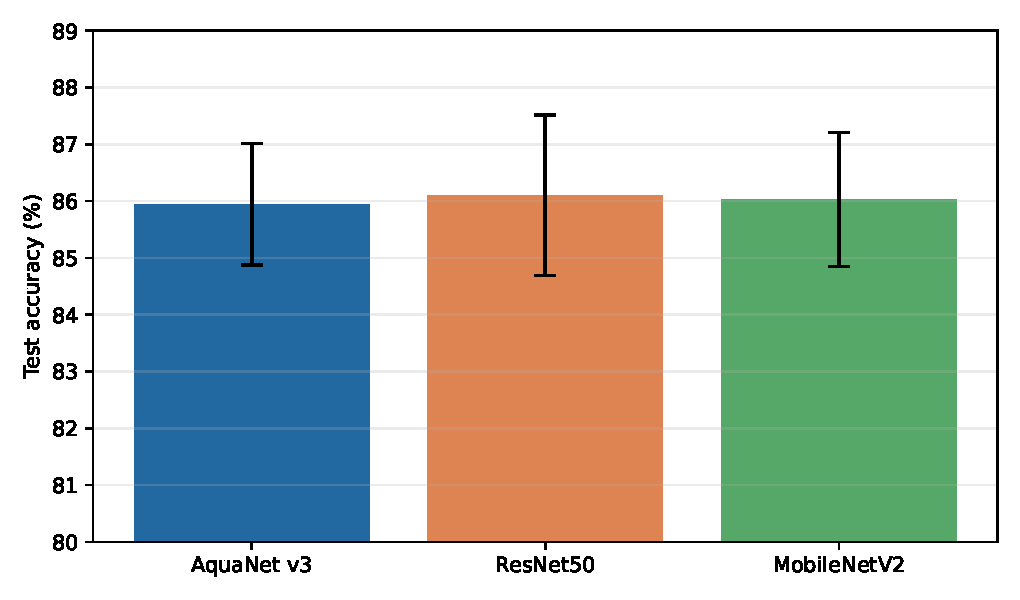
\includegraphics[width=\columnwidth]{figures/multiseed_accuracy.pdf}\caption{Mean D1 test accuracy over three matched seeds; error bars show sample standard deviation.}\label{fig:multi}\end{figure}
\begin{table*}[t]
\caption{Matched three-seed D1 results (mean $\pm$ sample standard deviation)}\label{tab:multi}\centering
\begin{tabular}{lrrrrrr}\toprule
Model & Accuracy (\%) & Macro-F1 & Weighted-F1 & ECE & NLL & Params (M)\\\midrule
AquaNet v3 & $85.95\pm1.07$ & $0.8233\pm0.0157$ & $0.8610\pm0.0115$ & $0.0655\pm0.0091$ & $0.4379\pm0.0334$ & 10.53\\
ResNet50 & $86.10\pm1.41$ & $0.8277\pm0.0152$ & $0.8643\pm0.0126$ & $0.0563\pm0.0145$ & $0.4226\pm0.0213$ & 23.52\\
MobileNetV2 & $86.03\pm1.18$ & $0.8292\pm0.0128$ & $0.8643\pm0.0123$ & $0.0595\pm0.0101$ & $0.4451\pm0.0362$ & 2.23\\\bottomrule
\end{tabular}
\end{table*}
Table~\ref{tab:multi} and Fig.~\ref{fig:multi} show near-identical mean accuracy. Relative to AquaNet v3, the paired accuracy difference is $-0.16$ percentage points versus ResNet50 ($p_t=0.914$, Wilcoxon $p=1.0$) and $-0.08$ points versus MobileNetV2 ($p_t=0.921$, Wilcoxon $p=1.0$). These runs provide no evidence of superiority. MobileNetV2 is also substantially smaller.

\subsection{Controlled substitutions}
\begin{figure}[t]\centering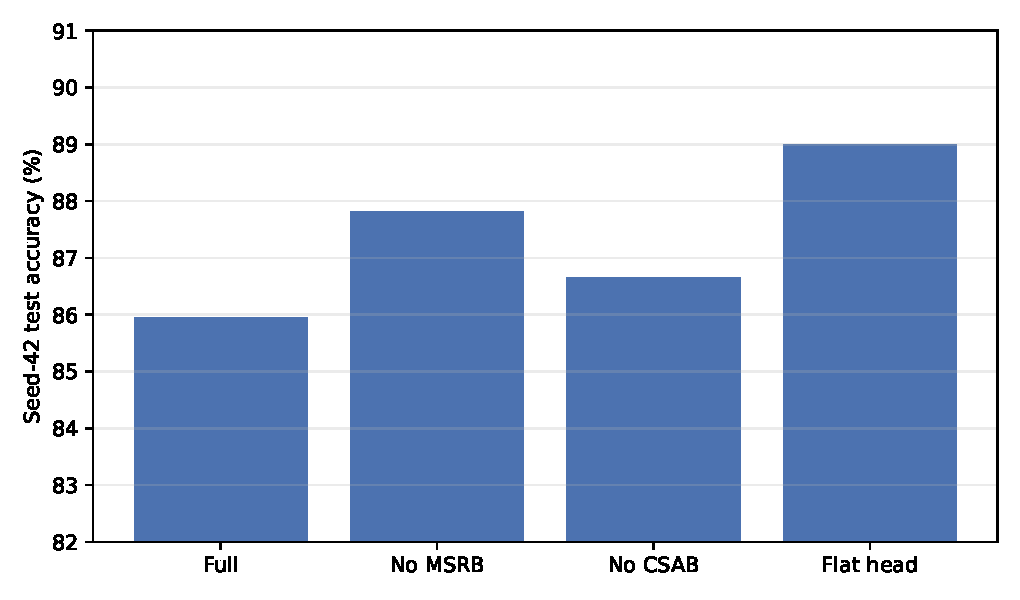
\includegraphics[width=\columnwidth]{figures/ablation_accuracy.pdf}\caption{Seed-42 controlled substitutions. These single-seed values are descriptive.}\label{fig:abl}\end{figure}
\begin{table}[t]
\caption{Seed-42 component substitutions}\label{tab:abl}\centering
\begin{tabular}{lrrr}\toprule
Variant & Acc. (\%) & Macro-F1 & NLL\\\midrule
Full & 85.71 & 0.8184 & 0.3994\\
No MSRB & 87.82 & 0.8404 & 0.3592\\
No CSAB & 86.65 & 0.8319 & 0.5065\\
Flat head & 88.99 & 0.8586 & 0.4182\\\bottomrule
\end{tabular}
\end{table}
The substitutions in Table~\ref{tab:abl} contradict a simple additive-benefit narrative. At seed 42, removing MSRB or hierarchical inference improves accuracy, while removing CSAB also exceeds the full model. NLL and accuracy do not rank all variants identically. Multiple-seed ablations are required before attributing causal benefit or harm.

\subsection{Class behavior and calibration}
\begin{figure}[t]\centering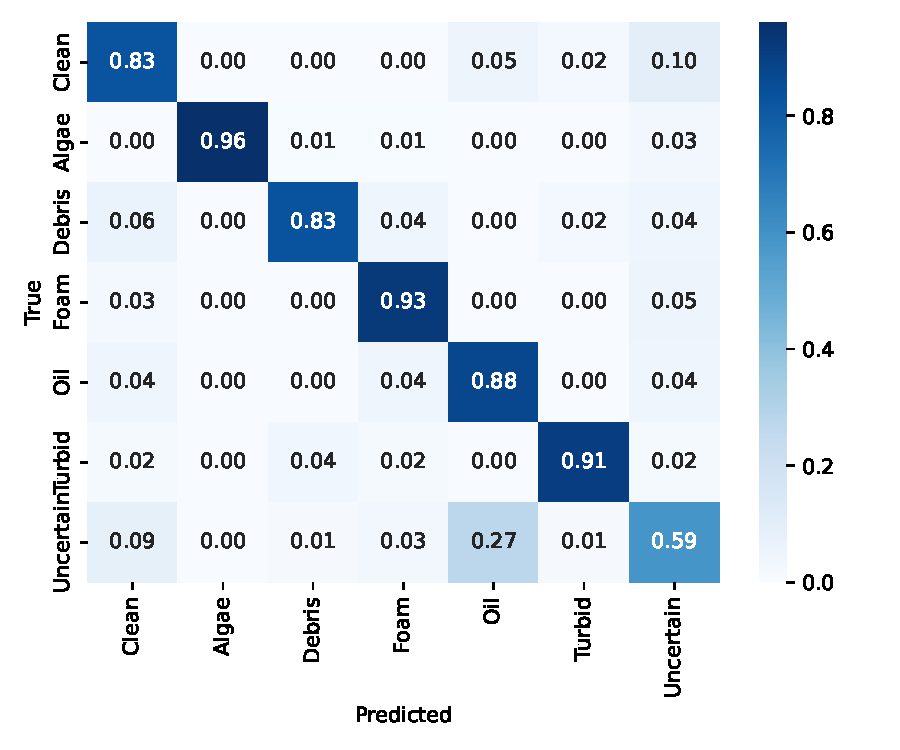
\includegraphics[width=\columnwidth]{figures/confusion_matrix.pdf}\caption{Normalized confusion matrix for the Phase-3 full model at seed 42.}\label{fig:cm}\end{figure}
The seed-42 full model reaches ECE 0.0556 and NLL 0.3994. Across seeds, its mean ECE is slightly worse than ResNet50 and MobileNetV2, providing no calibration advantage. Fig.~\ref{fig:cm} shows the corresponding class confusion pattern; conclusions about individual classes should be tempered by small support for oil and clean.

\subsection{Domain transfer}
\begin{figure}[t]\centering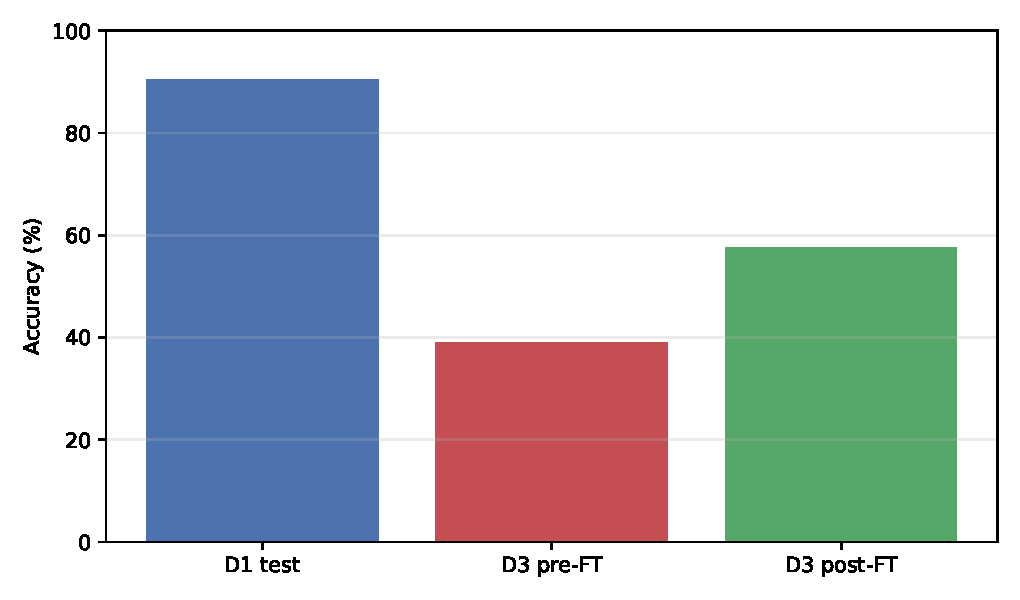
\includegraphics[width=\columnwidth]{figures/domain_transfer.pdf}\caption{Earlier retained AquaNet v3 benchmark and real-domain evaluation.}\label{fig:domain}\end{figure}
A retained earlier batch-64 seed-42 run, selected under its original protocol, reports 90.40\% on D1. Applied without real-image fine-tuning, it reaches 39.04\% on D3. Fine-tuning on D2 increases D3 accuracy to 57.53\%, an 18.49-point gain, but remains far below D1. The D2 validation split contains only 42 images and is image-level rather than source-video-grouped; its 90.48\% validation accuracy is therefore not treated as deployment evidence.

\section{Discussion}
The new protocol changes the interpretation in four ways. First, a single 90.40\% result is not representative of matched repeated training; checkpoint selection, batch size, and stochasticity matter. Second, matched means do not separate the proposed model from strong CNN baselines. Third, controlled substitutions do not validate the asserted contribution of each module. Fourth, the real-domain decline is larger than differences among benchmark architectures.

The work still offers useful engineering ideas: hierarchical probabilities encode a meaningful operational structure, MSRB exposes multiple receptive fields, and CSAB is inexpensive. But architectural plausibility is not empirical proof. Future work should use source-group splits, adjudicate perceptual candidates, repeat every ablation, tune all models under equal budgets, and evaluate a geographically distinct field dataset.

\section{Limitations}
The dataset provenance manifest and source-video identifiers are unavailable, preventing group-disjoint verification. dHash candidates have not been manually adjudicated. Only three repeated seeds and three baselines are included in Phase 3, and ablations have one seed. The latency measurements use shared-GPU batch execution and are suitable only for relative characterization, not edge deployment. D2 is small, and no ONNX, INT8, embedded-device, or canal-control experiment was performed. The study classifies visible appearance and does not measure physicochemical safety.

\section{Conclusion}
An evidence-first rebuild showed that AquaNet v3 does not significantly outperform ResNet50 or MobileNetV2 under a matched three-seed protocol. Single-seed substitutions likewise fail to establish that each proposed block improves performance. Exact duplicate screening is clean, but perceptual candidates and missing source groups prevent an absolute leakage-free claim. The strongest practical result is an 18.49-point improvement after real-image fine-tuning, alongside a large remaining domain gap. Reproducible evaluation and acquisition-aware splits are therefore more urgent than additional architectural complexity for this task.

\bibliographystyle{IEEEtran}
\bibliography{references}
\end{document}
